
\chapter{Skip Merger}
\label{chap:skipper}

\section{Theory}
The skip merger we introduce now uses the rather simple idea that if we consider classes of language equivalent states, then we only need to use the \enquote{last} SCC of those states and can remove all that come before.

\begin{defn}
	Let $\mathcal{A} = (Q, \Sigma, \delta, c)$ be a DPA and let $\sim \,\subseteq Q \times Q$ be a congruence relation on $\mathcal{A}$. Let $\preceq \,\subseteq Q \times Q$ be a total extension of $\preceq_\text{reach}^\mathcal{A}$. 
	
	We define the \emph{skip merger function} $\mu_\text{skip}^\sim : D \rightarrow 2^Q$ as follows: for each equivalence class $\kappa \in \mathfrak{C}(\sim)$, let $C_\kappa \subseteq \kappa$ be the of $\preceq$-maximal elements in $\kappa$. Let $M_\kappa = \kappa \setminus C_\kappa$. Then we have $D = \{ M_\kappa \mid \kappa \in \mathfrak{C}(\sim) \}$ and $\mu_\text{skip}^\sim(M_\kappa) = C_\kappa$.
\end{defn}

\vspace{5pt}

Now that we have established the definition of the merger, we want to analyze its structure and prove its correctness. For the rest of this section, we use $\mathcal{A} = (Q, \Sigma, \delta, c)$ as a DPA, $\sim$ as a congruence relation, and $\mathcal{B} = (Q_\mathcal{B}, \Sigma, \delta_\mathcal{B}, c_\mathcal{B})$ as a representative merge of $\mathcal{A}$ w.r.t. $\mu_\text{skip}^\sim$.

\begin{lem}
\label{lem:skip:run_growing}
	Let $\rho$ be a run on $\alpha$ in $\mathcal{B}$. Then for all $i$, $\rho(i) \preceq \rho(i+1)$.
	Furthermore, we have $\rho(i) \prec \rho(i+1)$ if and only if $\rho(i) \prec r_{[\delta(\rho(i), \alpha(i))]_\sim}$.
\end{lem}

\begin{proof}
	Let $i$ be an arbitrary index of the run. If $\rho(i)$ to $\rho(i+1)$ is also a transition in $\mathcal{A}$, then $\rho(i+1)$ is reachable from $\rho(i)$ in $\mathcal{A}$ and hence $\rho(i) \preceq \rho(i+1)$ by definition of the preorder. Otherwise the transition used was redirected in the construction. The way the redirection is defined, this implies $\rho(i) \prec \rho(i+1)$.
	
	We move on to the second part of the lemma. If $\rho(i) \prec r_{[\delta_\mathcal{A}(\rho(i), \alpha(i))]_\sim}$, then the transition is redirected to $\rho(i+1) = r_{[\delta_\mathcal{A}(\rho(i), \alpha(i))]_\sim}$ and the statement holds. 
	
	For the other direction, let $\rho(i) \prec \rho(i+1)$ and assume towards a contradiction that $\rho(i) \not\prec r_{[\delta_\mathcal{A}(\rho(i), \alpha(i))]_\sim}$. This means that the transition was not redirected and $\rho(i+1) = \delta_\mathcal{A}(\rho(i), \alpha(i))$. Since $\preceq$ is total, we have $r_{[\delta_\mathcal{A}(\rho(i), \alpha(i))]_\sim} = r_{[\rho(i+1)]_\sim} \preceq \rho(i) \prec \rho(i+1)$ which contradicts the $\preceq$-maximality of representatives.
\end{proof}

\begin{lem}
\label{lem:skip:equiv_same_scc}
	Let $p, q \in Q_\mathcal{B}$. If $p \sim q$, then $p$ and $q$ lie in the same SCC. 
\end{lem}

\begin{proof}
	It suffices to restrict ourselves to $q = r_{[q]_\sim} = r_{[p]_\sim}$. If we can prove the Lemma for this case, then the general statement follows by transitivity.
	
	Let $p_0$ be a state from which both $p$ and $q$ are reachable. Let $p_0 \cdots p_n$ be a minimal run of $\mathcal{B}$ that reaches $p$. By Lemma \ref{lem:skip:run_growing}, we have $p_0 \preceq \dots \preceq p_n$. Whenever $p_i \prec p_{i+1}$, a redirected transition to the representative $r_{[p_{i+1}]_\sim} = p_{i+1}$ is taken. 
	
	Let $k$ be the first position after which no redirected transition is taken anymore. For the first case, assume that $k < n$. Then $p_i \simeq r_{[p_{i+1}]_\sim}$ for all $i \geq k$. In particular, $p_{n-1} \simeq q$. Since $p_{n-1} \preceq p_n$, we also have $q \preceq p_n$. The representatives are chosen $\preceq$-maximal in their $\sim$-class, so $q \simeq p_n$.
	
	The second case is $k = n$. In that case, the transition from $p_{n-1}$ to $p_n$ is redirected and $p_n = r_{[p_n]_\sim} = q$.
\end{proof}


\begin{lem}
\label{lem:skip:run_suffix}
	Let $\rho \in Q^\omega$ be an infinite run in $\mathcal{B}$. Then $\rho$ has a suffix that is a run in $\mathcal{A}$.
\end{lem} 

\begin{proof}
	We show that only finitely often a redirected transition is used in $\rho$. Then, from some point on, only transitions that also exist in $\mathcal{A}$ are used. The suffix starting at this point is the run that we are looking for.
	
	Let $\rho = p_0 p_1 \cdots$. By Lemma \ref{lem:skip:run_growing}, we have $p_i \preceq p_{i+1}$ for all $i$ and $p_i \prec p_{i+1}$ whenever a redirected transition is taken. As $Q$ is finite, we can only move up in the order finitely often. This proves our claim.
\end{proof}


\begin{theorem}
	Let $\sim \,\subseteq\, \equiv_L$. Then $\mathcal{A}$ and $\mathcal{B}$ are language equivalent.
\label{thm:skip:lang_equiv}
\end{theorem}

\begin{proof}
	Let $\alpha \in \Sigma^\omega$ be a word and let $\rho$ be of $\mathcal{B}$ starting in $q_0$ on $\alpha$. By Lemma \ref{lem:skip:run_suffix}, $\rho$ has a suffix $\pi$ which is a run segment of $\mathcal{A}$ on some suffix $\beta$ of $\alpha$. The acceptance condition of DPAs is prefix independent, so $\alpha \in L(\mathcal{B}, q_0)$ iff $\rho$ is an accepting run iff $\pi$ is an accepting run. Since the priorities do not change during the construction, $\pi$ is accepting in $\mathcal{B}$ iff it is accepting in $\mathcal{A}$.
	
	Let $w \in \Sigma^*$ be the prefix of $\alpha$ with $\alpha = w \beta$. By Lemma \ref{lem:general:cong_stays_in_merge}, we know that $\delta^*(q_0, w) \sim \delta^*_\mathcal{B}(q_0, w)$. Since every state is $\sim$-equivalent to its representative and $\sim$ is a congruence relation, we also know $\delta^*_\mathcal{B}(q_0, w) \sim \delta^*_\mathcal{B}(r_{[q_0]_\sim}, w)$. From $\delta^*_\mathcal{B}(r_{[q_0]_\sim}, w)$, the run $\pi$ accepts $\beta$ iff $\alpha \in L(\mathcal{B}, q_0)$. As $\sim$ implies language equivalence, the same must hold for $\delta^*_\mathcal{A}(q_0, w)$. Therefore, $\alpha \in L(\mathcal{A}, q_0)$ iff $\alpha \in L(\mathcal{B}, q_0)$.
\end{proof}




\section{Computation}

\begin{lem}
\label{lem:skip:skip_aut_linear_time}
	For a given $\mathcal{A}$ and $\sim$, $\mu_\text{skip}^\sim$ can be computed in $\mathcal{O}(|\mathcal{A}|)$.
\end{lem}

\begin{proof}
	As seen in Lemma \ref{lem:general:reach_topo_lintime}, $\preceq$ can be computed in linear time. Assuming that $\sim$ is given by a suitable data structure, each equivalence class can easily be accessed and $\preceq$-maximal elements can be found in linear time.
\end{proof}





\section{Efficiency}
%TODO

\begin{figure}
	\centering
	\begin{minipage}{0.49\textwidth}
		\includegraphics[page=6,height=.3\textheight]{../data/analysis/skipper/gendet_ap1.pdf} 
		\includegraphics[page=6,height=.3\textheight]{../data/analysis/skipper/detspot_ap1.pdf} 
		\includegraphics[page=6,height=.3\textheight]{../data/analysis/skipper/detnbaut_ap1.pdf} 
		\caption{Relative state reduction of different automata using $\mu_\text{skip}^{\equiv_\text{\Ankh}}$.}
		\label{fig:skip:empirical_size_hist}
	\end{minipage}
	\hfill
	\begin{minipage}{0.49\textwidth}
		\includegraphics[page=2,height=.3\textheight]{../data/analysis/skipper/gendet_ap1.pdf} 
		\includegraphics[page=2,height=.3\textheight]{../data/analysis/skipper/detspot_ap1.pdf} 
		\includegraphics[page=2,height=.3\textheight]{../data/analysis/skipper/detnbaut_ap1.pdf} 
		\caption{Relative state reduction of different automata using $\mu_\text{skip}^{\equiv_\text{\Ankh}}$.}
		\label{fig:skip:empirical_reduct_abs}
	\end{minipage}
\end{figure}